% Use class option [extendedabs] to prepare the 1-page extended abstract.
\documentclass[extendedabs]{bmvc2k}
\usepackage[colorlinks = true,
            linkcolor = blue,
            urlcolor  = blue,
            citecolor = blue,
            anchorcolor = blue]{hyperref}

\usepackage{kotex}
% for the fancy \koTeX logo
\usepackage{kotex-logo}

% Document starts here
\begin{document}


\title{YOLO final-report}
\addauthor{
김태훈$^{1}$
}{}{1}

\addinstitution{
$^1$부산대학교 전기컴퓨터공학부.  
}
 
\maketitle
\noindent

\section{Introduction}
YOLO\cite{yolopaper} is the object detection model that detect object using a single neural-network regression of spatially separated bounding boxes and associated class probabilities. the paper\cite{yolopaper} says YOLO is extremly fast(45 frames per second) while achieving double the mAP of other real-time object detection like Fastest DPM\cite{fastestdpm}.

In this report, We use Pytorch to implement YOLO, we use PASCAL VOC 2007 and 2012\cite{pascalvoc} dataset to training the model, and we will analyze and discuss the training and inference results.

\section{Dataset}
As mentioned before, we use PASCAL VOC 2007 and 2012\cite{pascalvoc} dataset for training, and PASCAL VOC 2007test dataset for testing. there are 4300 images for training, and 1227 for testing. there are 6 categories(aeroplane, bicycle, bus, car, cat, dog) in the dataset. the Labeling data are consist of objects category and coordinate(xmin, ymin, xmax, ymax)

\subsection{Pre-processing}
We increase the image size from $224\times224$ to $448\times448$ same as the paper.\cite{yolopaper}

For data augmentation, Each image was horizontal flipped, resized(0.8 to 1.2), shifted, cropped with a 50\% chance. Also, changing brightness, saturation, hue of the image and blurring it were processed with a 50\% chance. Labeling data are also changed when corresponding image was changed.

\begin{figure}[t]
	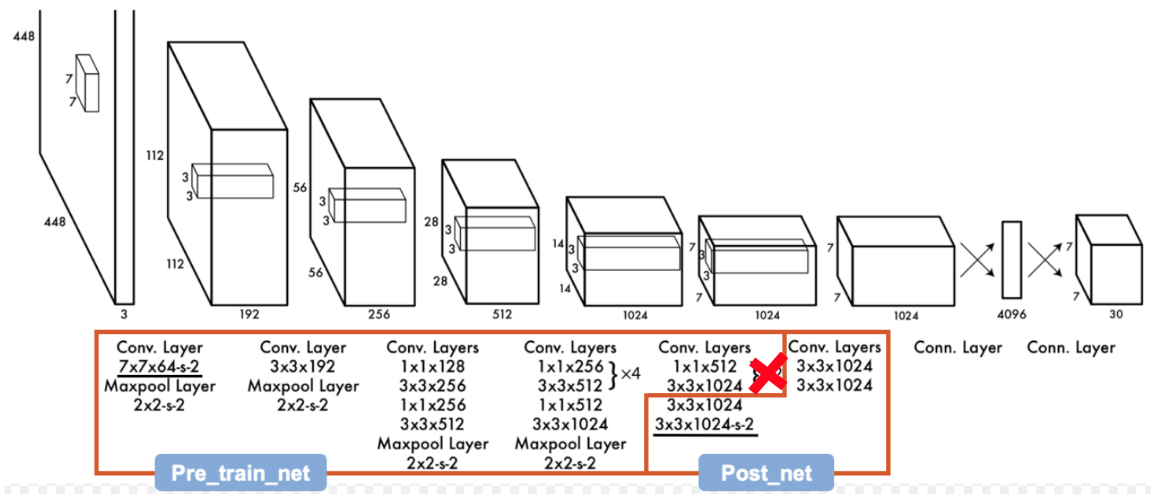
\includegraphics[width=\linewidth]{images/architecture.png}
	\caption{
		Architecture of the YOLO model. Our network has 22 convolutional layers followed by 2 fully connected layers. $1\times1$ convolutional layers reduce the features space}
	\vspace{-2mm}
        \label{fig:netarch}
\end{figure}

\section{Network Architecture}
Our network has 22 convolution layers followed by 2 Fully-connected layers, which is slightly different from the paper\cite{yolopaper}'s architecture that has 24 convolution layers followed by 2 fully-connected layers. Our network has 22 Convolutional layers, 4 Max Pooling layers, 2 Fully connected layers. The activation function of this model is Leaky ReLU with 0.1 negative slope. The full network is shown in Figure \ref{fig:netarch}.
 
The output shape of the model is $7\times\ 7\times 30$. the $7\times 7$ means the input image is divided into an $7\times7$ grid of cells. and $30$ means Each grid cell predict 2 bounding boxes and 20 classes probabilities. Each bounding box consists of x,y, width, height, and confidence score. (x,y) coordinates mean the center of the box relative to the top-left bounds of the grid cell. The width and height are relative to the whole image.

The target confidence score is zero if there are no objects in that cell. If the cell contains objects, the confidence score is equal to the intersection over union between predicted box and the ground truth.

the YOLO and YOLO vanila model has about 266M parameters, and YOLO VGG-16 has about 260M parameters.

\section{Loss function}
The loss function of the model is shown in Figure \ref{fig:loss}, where $\textbf{1}^{obj}_i$ denotes whether object appears in cell and $\textbf{1}^{obj}_{ij}$ denotes that the $j$th bounding box predictor in cell $i$ is responsible for that prediction. the "responsible" bounding boxes has highest IOU with the ground truth. Also, $\lambda_{coord}$ is balancing parameter for increasing the loss from bounding box coordinate than classification, and $\lambda_{noobj}$ is for decreasing loss from confidence score of grid that don't contain objects. The error function is sum-squared error.

The meaning of each term is as follows:

\begin{enumerate}
  \item For the responsible bounding box predictor $j$ in cell $i$ that containing object, get loss of coordinate of center of the bounding box.
  \item For the responsible bounding box predictor $j$ in cell $i$ that containing object, get loss of square root of width and height
  \item For the responsible bounding box predictor $j$ in cell $i$ that containing object, get loss of confidence score ($C_i=1$)
  \item For the responsible bounding box predictor $j$ in cell $i$ that don't contain object, get loss of confidence score ($C_i=0$)
  \item For cell that contains object, get loss of class probabilities.
\end{enumerate}

\begin{figure}[t]
	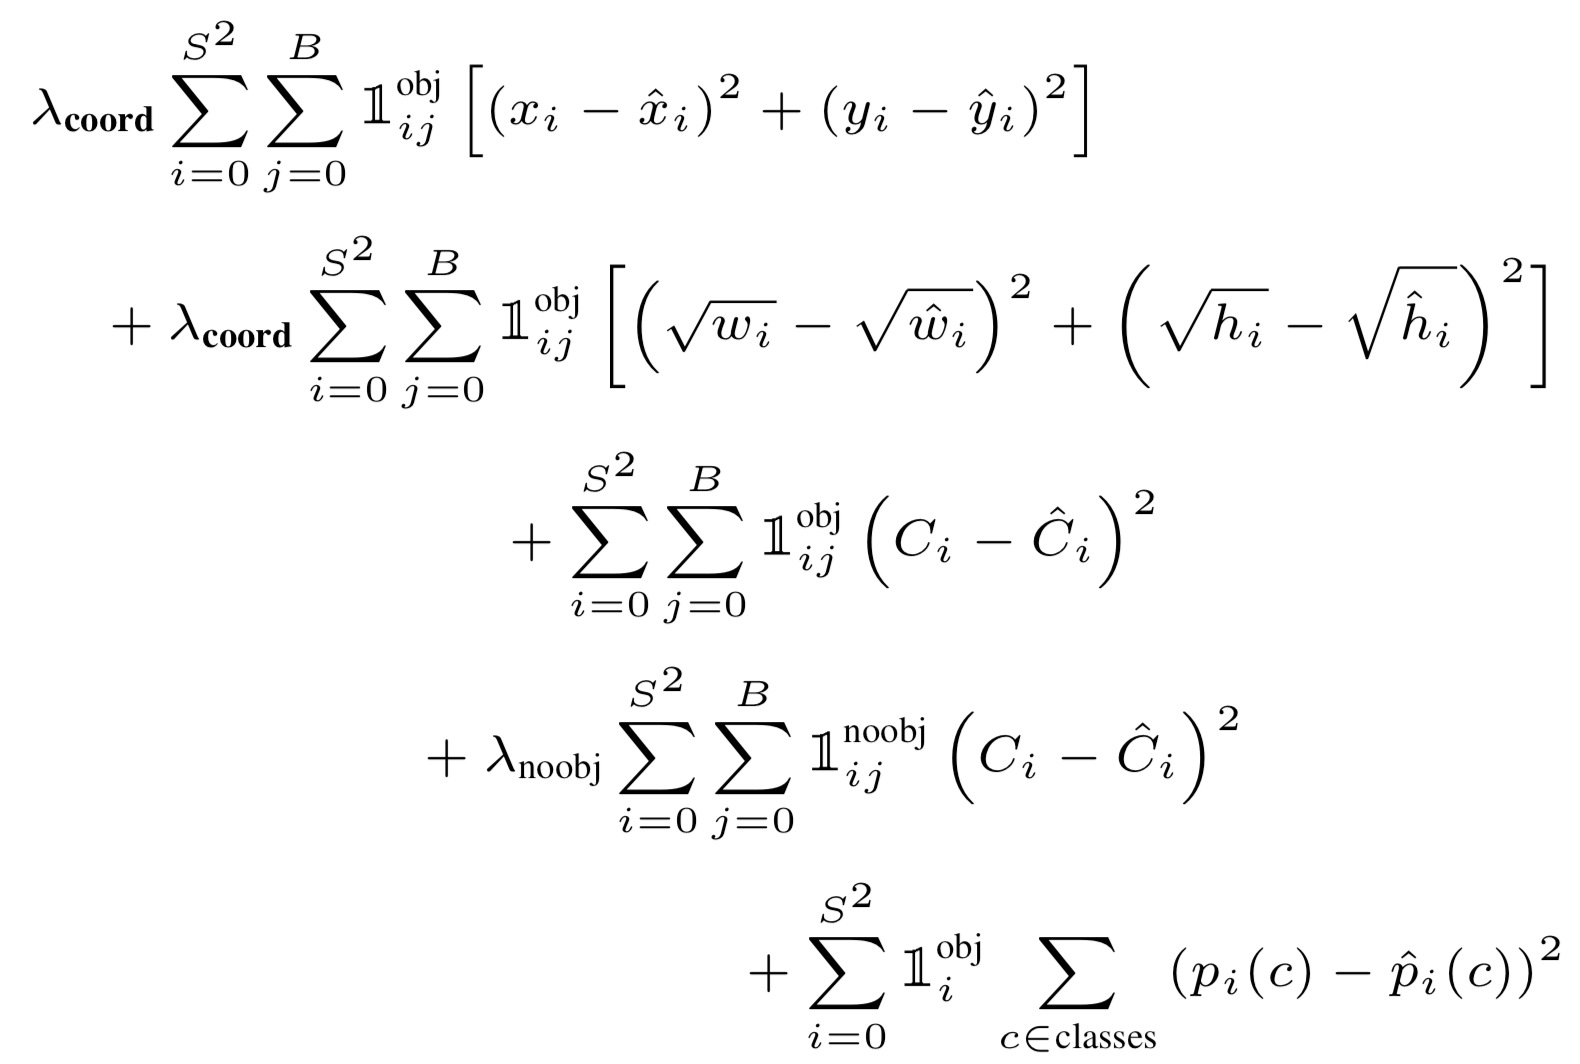
\includegraphics[width=\linewidth]{images/loss.png}
	\caption{
		Loss function of the YOLO model.}
	\vspace{-2mm}
        \label{fig:loss}
\end{figure}

The above loss functions are in the paper\cite{yolopaper}. however, Our loss function is little different from the paper\cite{yolopaper}. First, We get loss for the bounding box predictor $j$ in cell $i$ that don't contain object, not "responsible" bounding box. Also, We use mean-squared error for YOLO in Table \ref{tab:models}  because the loss exploded to nan after applying sum-squared error and pre-train weights.

\section{Training}
We set two parameters $\lambda_{coord}=5$ and $\lambda_{noobj}=0.5$. We train 3 slightly different model for comparison. explanation of the each model is shown in Table \ref{tab:models}

\begin{table}[]
\centering
\begin{tabular}{|l|l|l|}
\hline
model name  & pre-trained                                                                                                            & error \\ \hline
YOLO        & \begin{tabular}[c]{@{}l@{}}all layers are pre-trained with \\ 68.5mAP performance weights\end{tabular}                & MSE   \\ \hline
YOLO VGG-16 & \begin{tabular}[c]{@{}l@{}}first 18 convolution layers are changed to \\ VGG-16\cite{vggnetpaper} pre-trained with Imagenet\end{tabular} & SSE   \\ \hline
YOLO vanila & all layers are not pre-trained                                                                                         & SSE   \\ \hline
\end{tabular}
\caption{The explanation of the models. SSE means Sum-Squared error, MSE means Mean-Squared error}
\label{tab:models}
\end{table}

We train the networks for 15 epochs with 10 batch size, $10^{-4}$ learning rate and $5\times10^{-4}$ weight decay. Learning rate is fixed to $10^{-4}$ during training.

\section{Experiment}

\begin{table}[]
\centering
\begin{tabular}{l|l|llllll}
            & mAP  & aero & bike & bus  & car  & cat  & dog  \\ \hline
YOLO        & 62.6 & 59.4 & 62.0 & 52.0 & 61.4 & 69.7 & 71.3 \\
YOLO VGG-16 & 30.0 & 36.6 & 40.4 & 0.0  & 34.5 & 38.2 & 30.4 \\
YOLO vanila & 4.4 & 6.4 & 0.0  & 0.0  & 2.0  & 0.3 & 17.6 
\end{tabular}
\caption{The average precision of the models after training. Each value is rounded off to the first decimal place. The test dataset is PASCAL VOC 2007test.}
\label{tab:results}
\end{table}

\begin{figure}[t]
	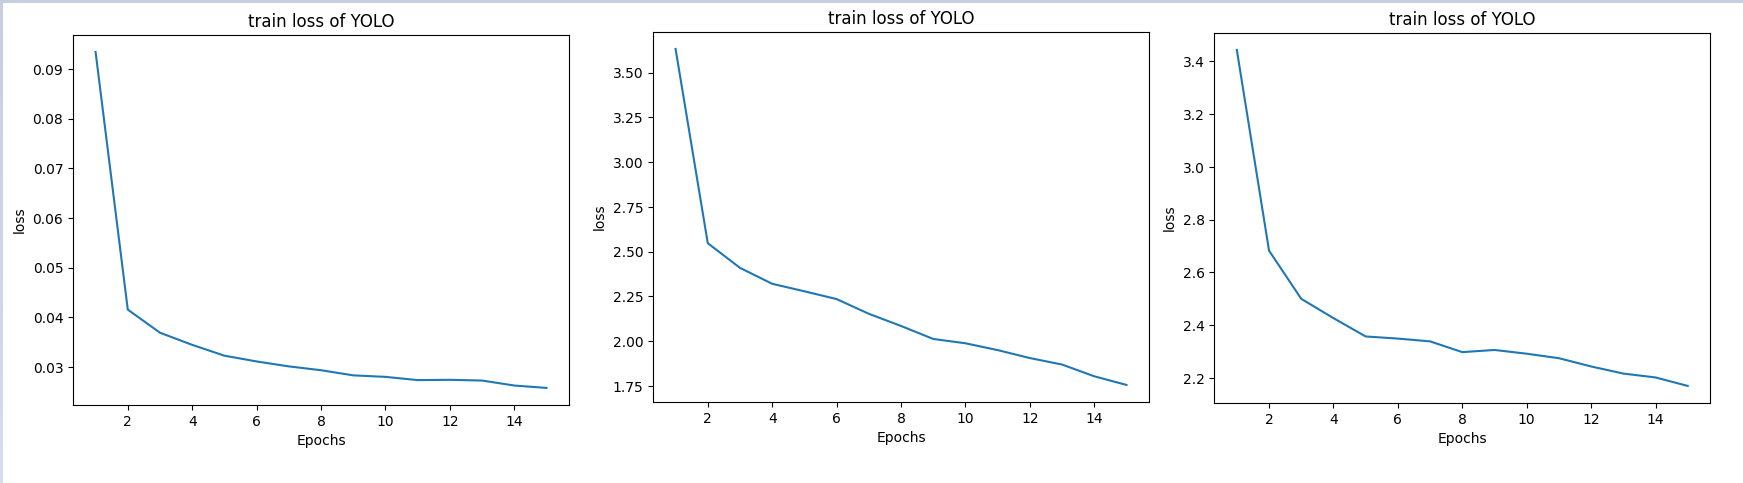
\includegraphics[width=\linewidth]{images/losschart.PNG}
	\caption{Training loss of the each model. The left is YOLO, the middle is YOLO VGG-16, and right is YOLO vanila.
		}
	\vspace{-2mm}
        \label{fig:losschart}
\end{figure}

\begin{figure}[t]
	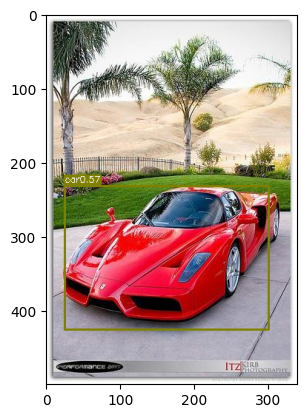
\includegraphics[width=0.5\linewidth]{images/infercar.png}
	\caption{Visualizing result of the YOLO model using a car image.
		}
	\vspace{-2mm}
        \label{fig:infercar}
\end{figure}

After training, We test the models with PASCAL VOC 2007test dataset. The results of each model are shown in Table \ref{tab:results}. the mAP of the YOLO model is 62.6, YOLO VGG-16 is 30.0, YOLO vanila is 4.4.

\subsection{Discussion}
The mAP of the YOLO model is less than pre-trained model. this may be because the construction of the loss function is wrong and applying mean-squared error function. We tried to apply pre-trained weights and sum-squared error same as the paper\cite{yolopaper}, but we struggle to apply it because the loss is exploded to nan. So We apply MSE error function as stopgap. We will find a solution after the report. but the mAP is 62.6, which is better than other real-time object detection model like DPM\cite{dpm}.

the mAP of YOLO VGG-16 is 30.0, which significantly lower than the YOLO VGG-16 of the paper\cite{yolopaper}. this may be because 15 epochs is too smaller than 135 epochs of the paper\cite{yolopaper}.

the mAP of YOLO vanila is the lowest among the models. this is because all layers are not pre-trained. 4300 images is insufficient to train all parameters in the model. The paper\cite{yolopaper} pretrained first 20 convolution layers with Imagenet dataset. 

\section{Conclusion}
We implemented YOLO, object detection model using regression with single neural network. We confirm that the YOLO has quite good performance despite it uses single neural network Unlike other object detection model like Fast R-CNN\cite{fastrcnn}. If we solve the nan loss problem, we will be able to confirm better on this model.

\newpage
\bibliography{egbib}

\end{document}
